\chapter{نمودارهای کلاس طراحی}
({\color{red} بهنگام‌سازی شد.}) \\
در این فصل نمودارهای کلاس طراحی همراه با جزییات آن‌ها آورده شده است. به علت جلوگیری از ناخوانا شدن، از مکانیزم بسته‌بندی
\LTRfootnote{Packaging}
استفاده شده است. در هر بسته چند کلاس مرتبط به همراه ارتباطهایشان با کلاس‌های بیرونی قابل مشاهده است.
\begin{landscape}
	\section{بسته پروژه}
	\begin{figure}[H]
		\centering
		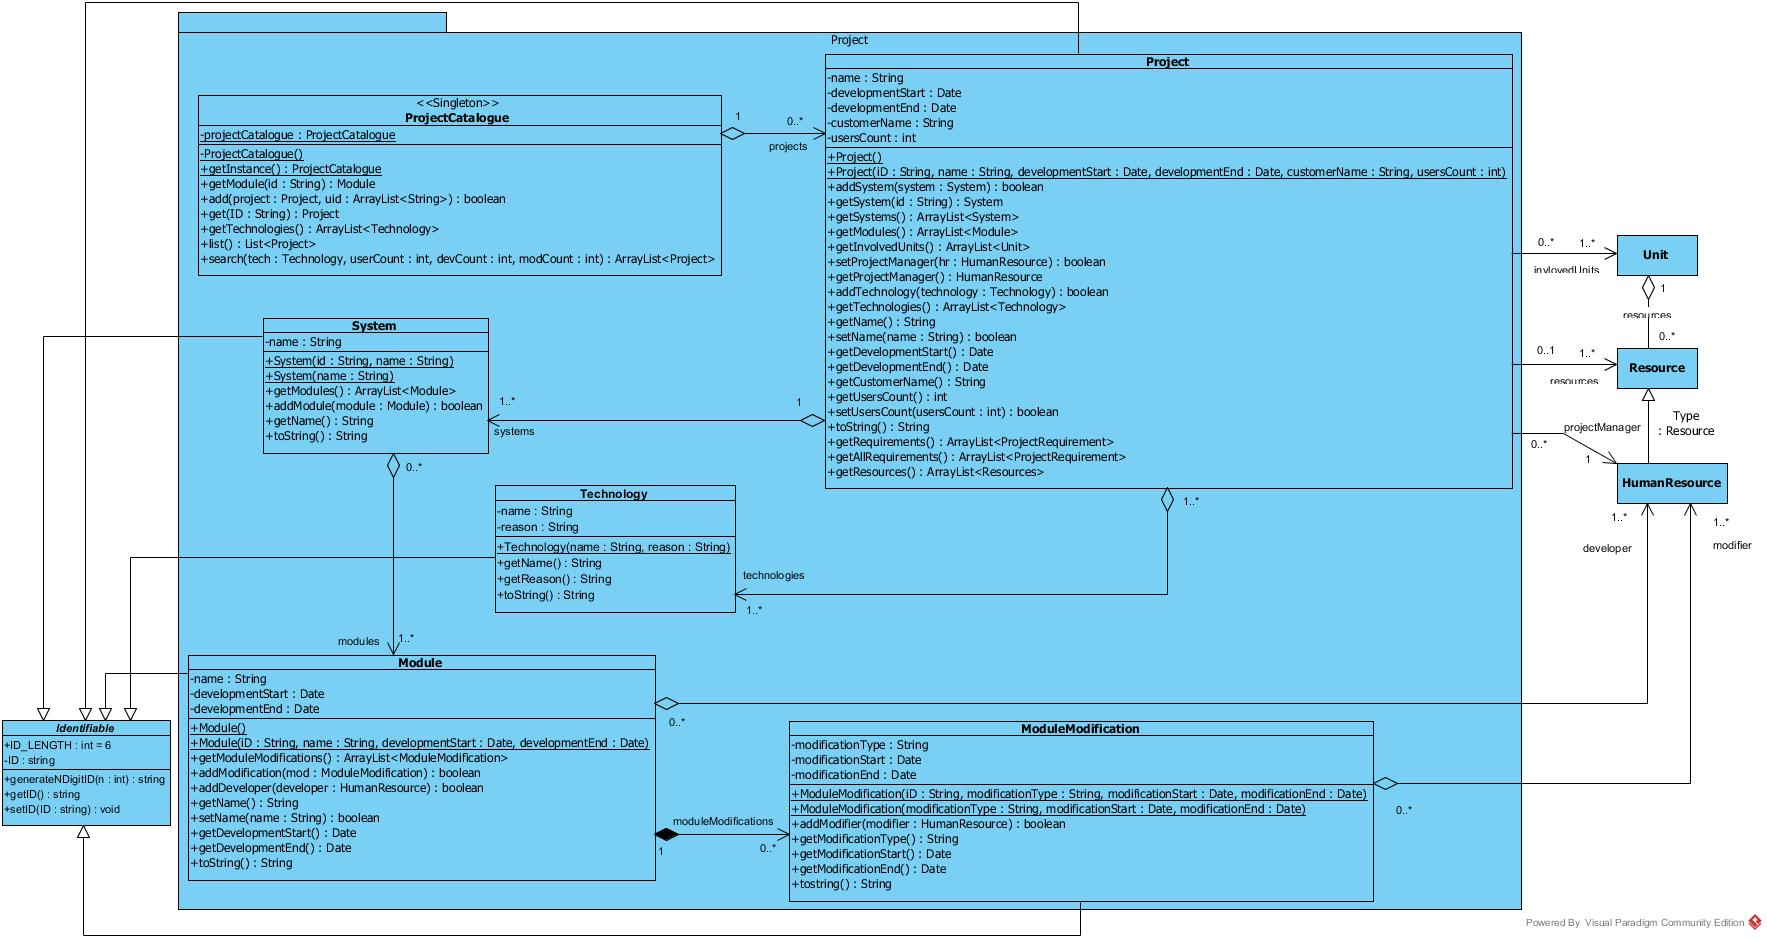
\includegraphics[scale=0.4]{img/class-design/ProjectPackage}
		\caption{بسته پروژه}
	\end{figure}
	
	
	
	\section{بسته منبع}
	\begin{figure}[H]
		\centering
		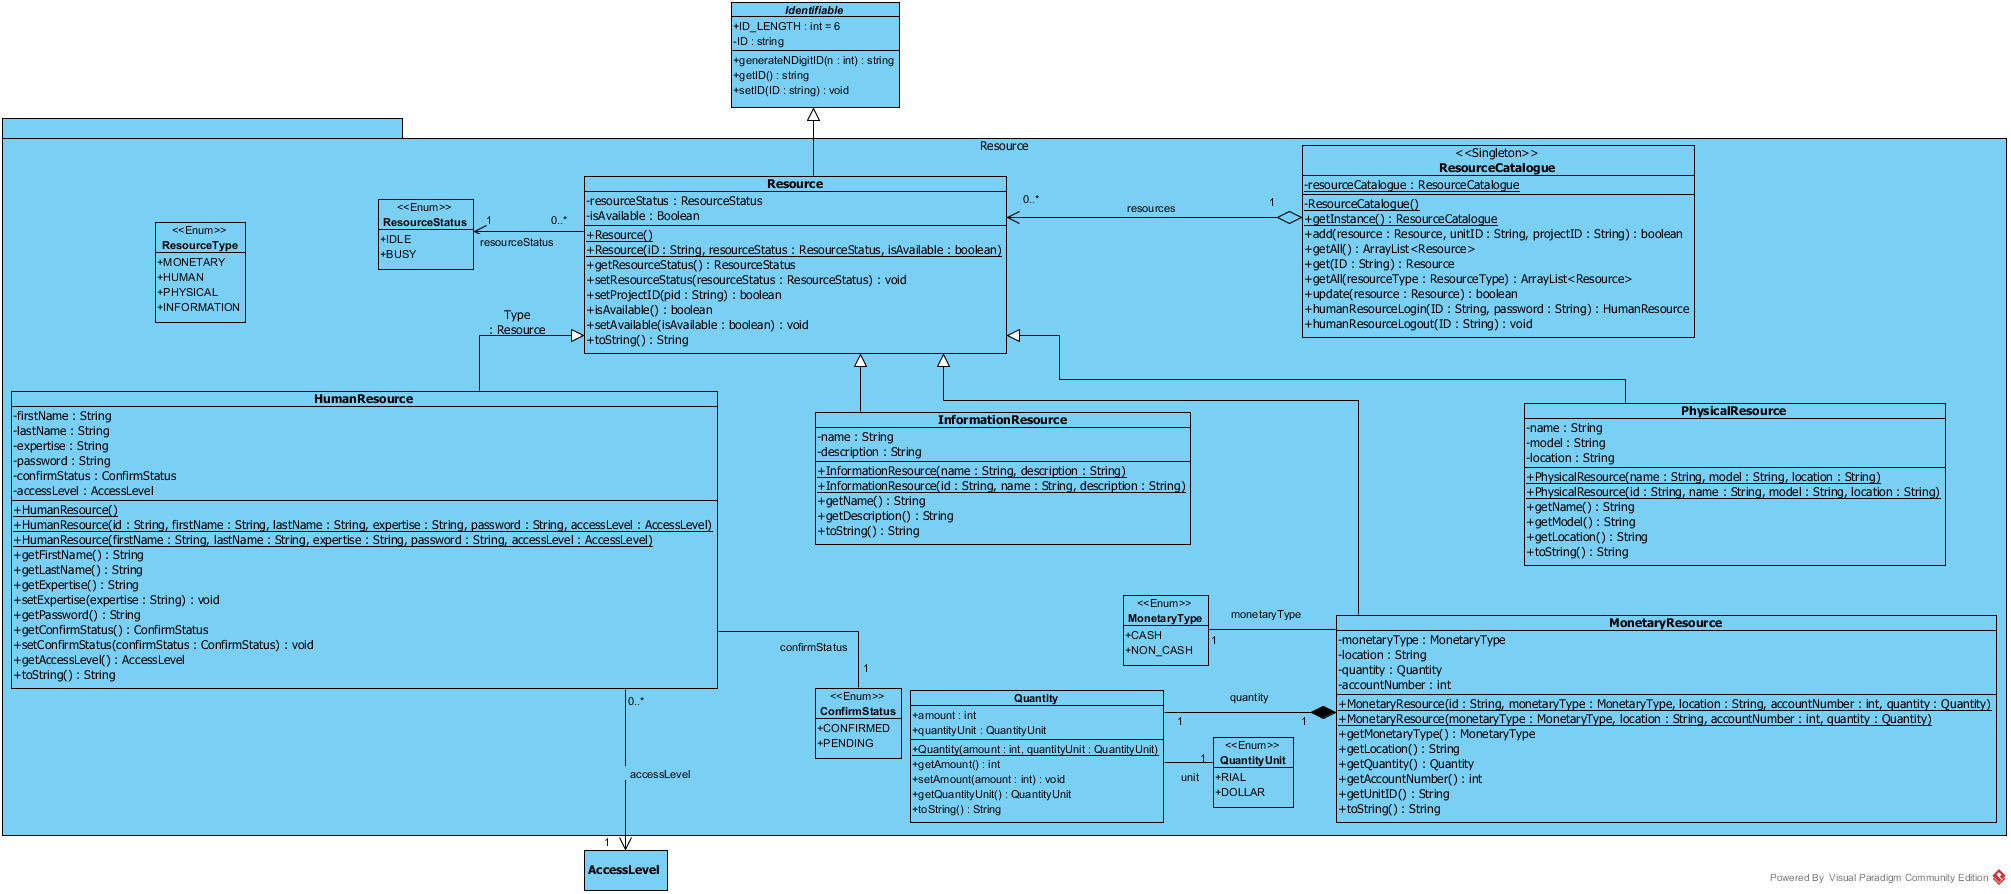
\includegraphics[scale=0.45]{img/class-design/ResourcePackage}
		\caption{بسته منیع}
	\end{figure}
	
	
	\section{بسته واحد}
	\begin{figure}[H]
		\centering
		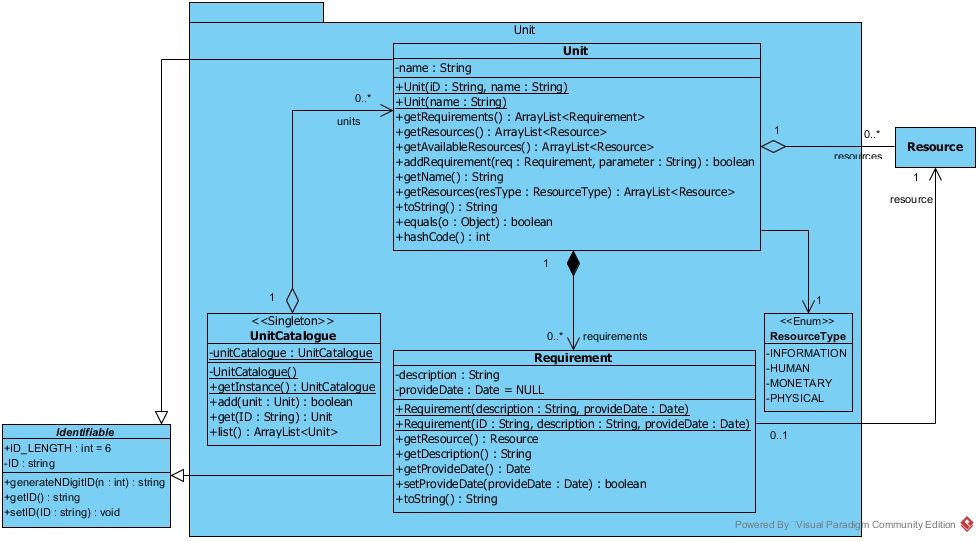
\includegraphics[scale=0.6]{img/class-design/UnitPackage}
		\caption{بسته واحد}
	\end{figure}
	
	\section{بسته گزارش}
	\begin{figure}[H]
		\centering
		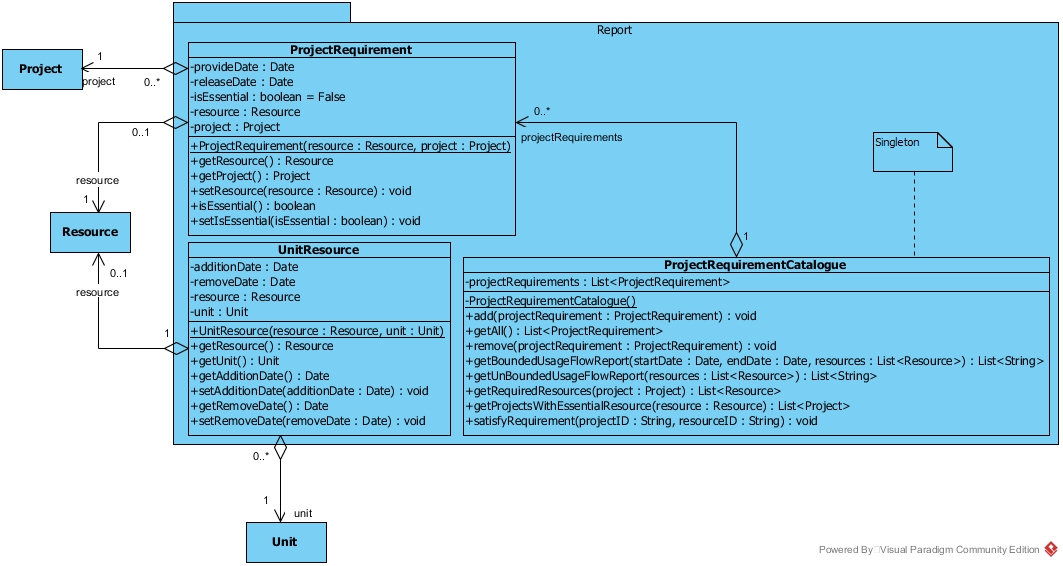
\includegraphics[scale=0.45]{img/class-design/ReportPackage}
		\caption{بسته گزارش}
	\end{figure}
	
	\section{بسته دسترسی}
	\begin{figure}[H]
		\centering
		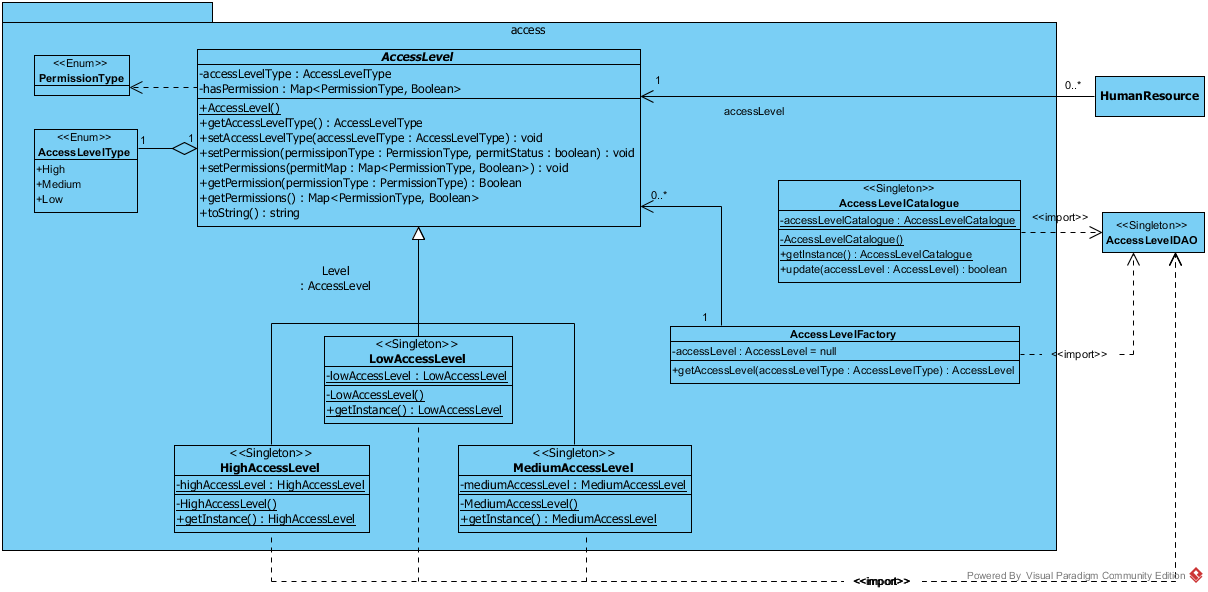
\includegraphics[scale=0.6]{img/class-design/AccessPackage}
		\caption{بسته دسترسی}
	\end{figure}
	
	\newpage
	\section{بسته ارتباط لایه منطق و لایه نمایش }
	کلاس‌های Facade با توجّه به کاربردشان با برخی از کلاس‌های دیگر ارتباط از نوع instantiate دارند که به منظور جلوگیری از ازدحام نمودار، تنها ا
	رتباط کلاس‌های OperationFacade ، UserFacade و ProjectFacade با کلاس‌های کاتالوگ کشیده شده است.
	\begin{figure}[H]
		\centering
		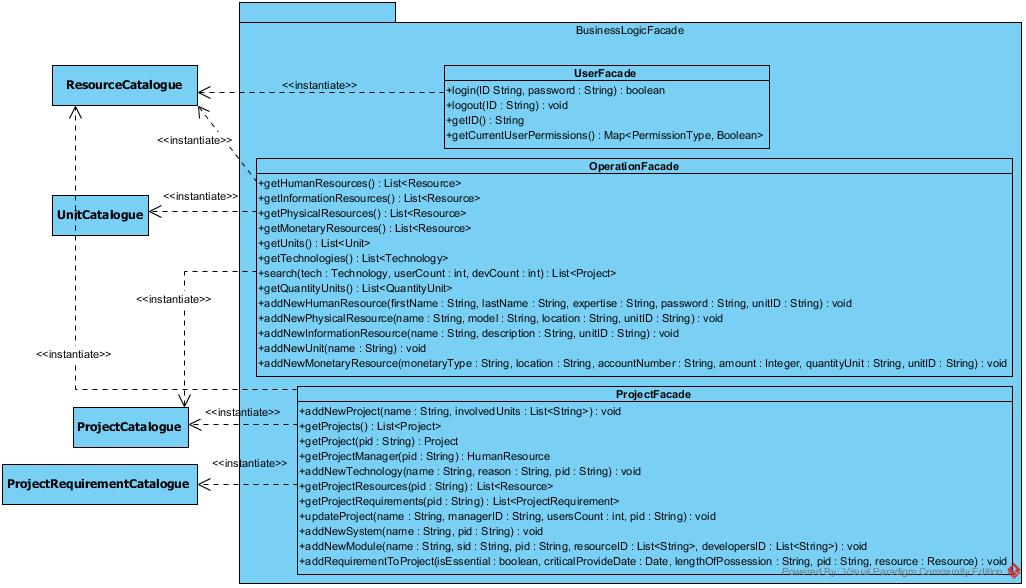
\includegraphics[scale=0.5]{img/class-design/BusinessLogicFacade}
		\caption{بسته ارتباط لایه منطق و لایه نمایش}
	\end{figure}
	
	
	\newpage
	\section{بسته پایگاه‌داده}
	از آن‌جایی که کلاس قالب
	\LTRfootnote{Template}
	DAO یک واسط است، لازم است که توابع آن در همه‌ی کلاس‌هایی که به آن bind می‌شوند پیاده‌سازی شود. اما با توجه به ملاحظات مربوط به خوانایی و قرارگیری در مستند، از تکرار آن‌ها در کلاس‌های با پسوند DAO خودداری شده است.
	\\
	همچنین، کلاسی تحت نام QueryGenerator استفاده شده است که Singleton است و توابع موجود در دیگر کلاس‌های این بسته از آن استفاده کرده‌اند تا نیازی نباشد هربار پرسمان SQL به طور کامل نوشته شود. ارتباط‌های از نوع use که بین این کلاس و دیگر کلاس‌ها وجود دارد، جهت خوانایی آورده نشده است.
	\begin{figure}[H]
		\centering
		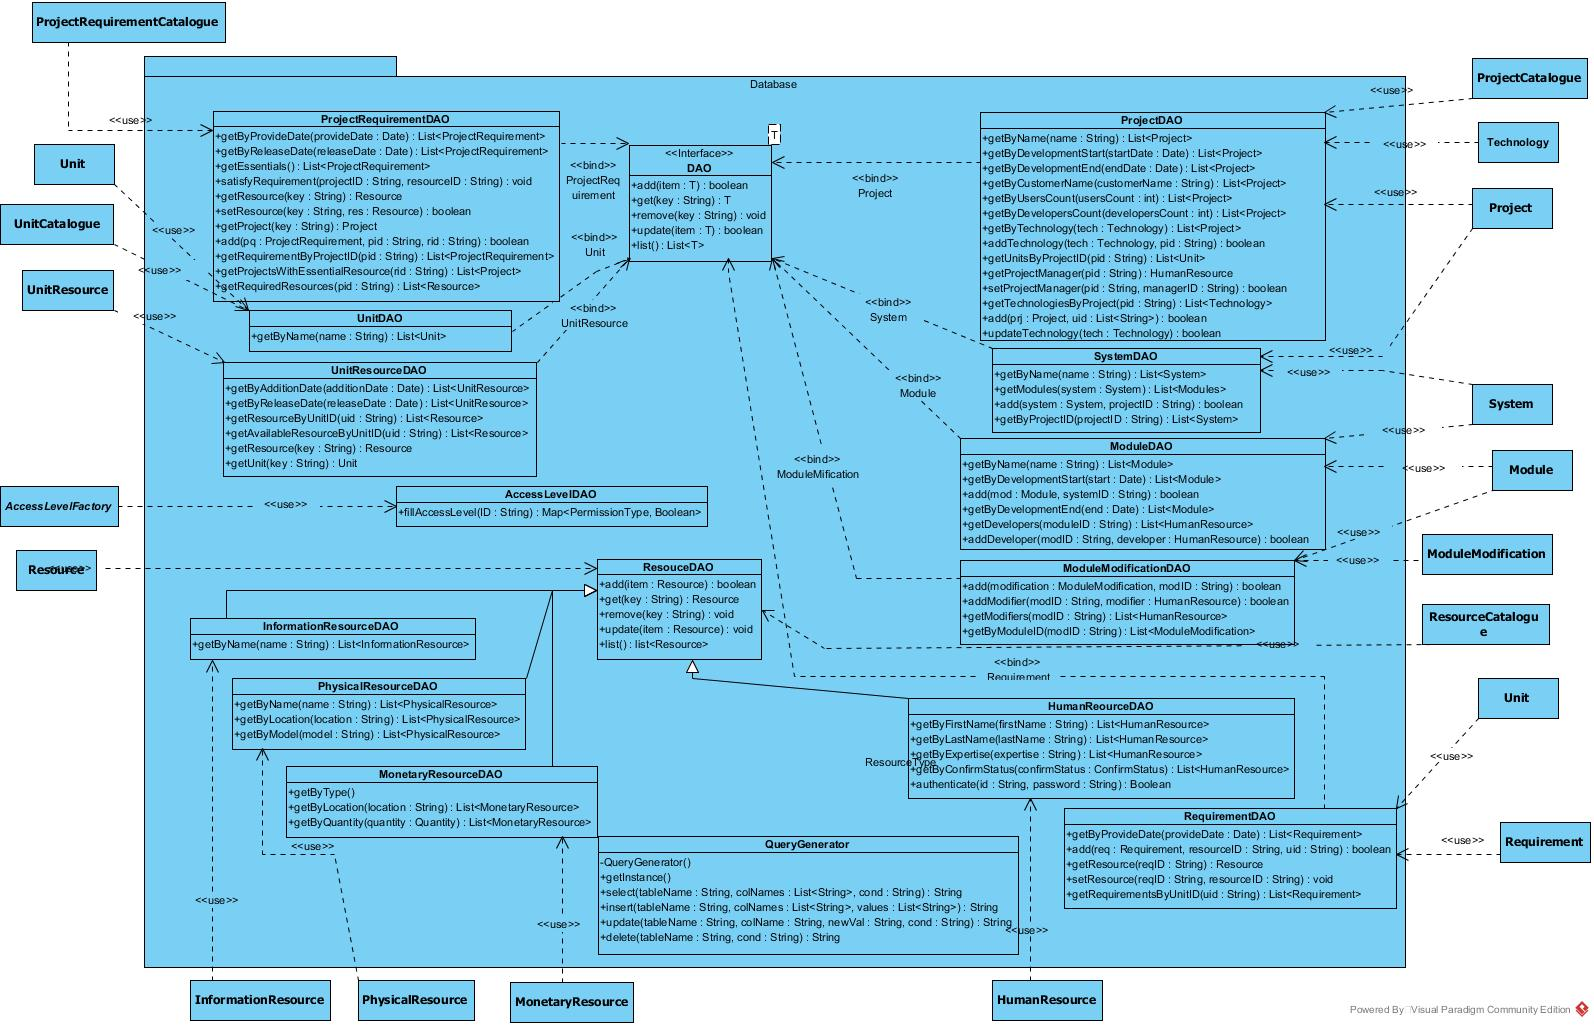
\includegraphics[scale=0.4]{img/class-design/DatabasePackage}
		\caption{بسته پایگاه‌داده}
	\end{figure}
\end{landscape}


\begin{landscape}
	\section{کلاس‌های واسط کاربری}
	\subsection{نمای کلی کلاس‌های واسط کاربری}
	به منظور جلوگیری از شلوغی و دشوار‌فهم شدن نمودارها، در نمودار زیر تنها روابط وراثت و تحقّق بین کلاس‌ها و واسط‌ها نمایش داده شده است. جزئیات تمام کلاس‌ها در ادامه در بسته‌های جداگانه نمایش داده خواهد شد.\\
	\begin{figure}[H]
		\centering
		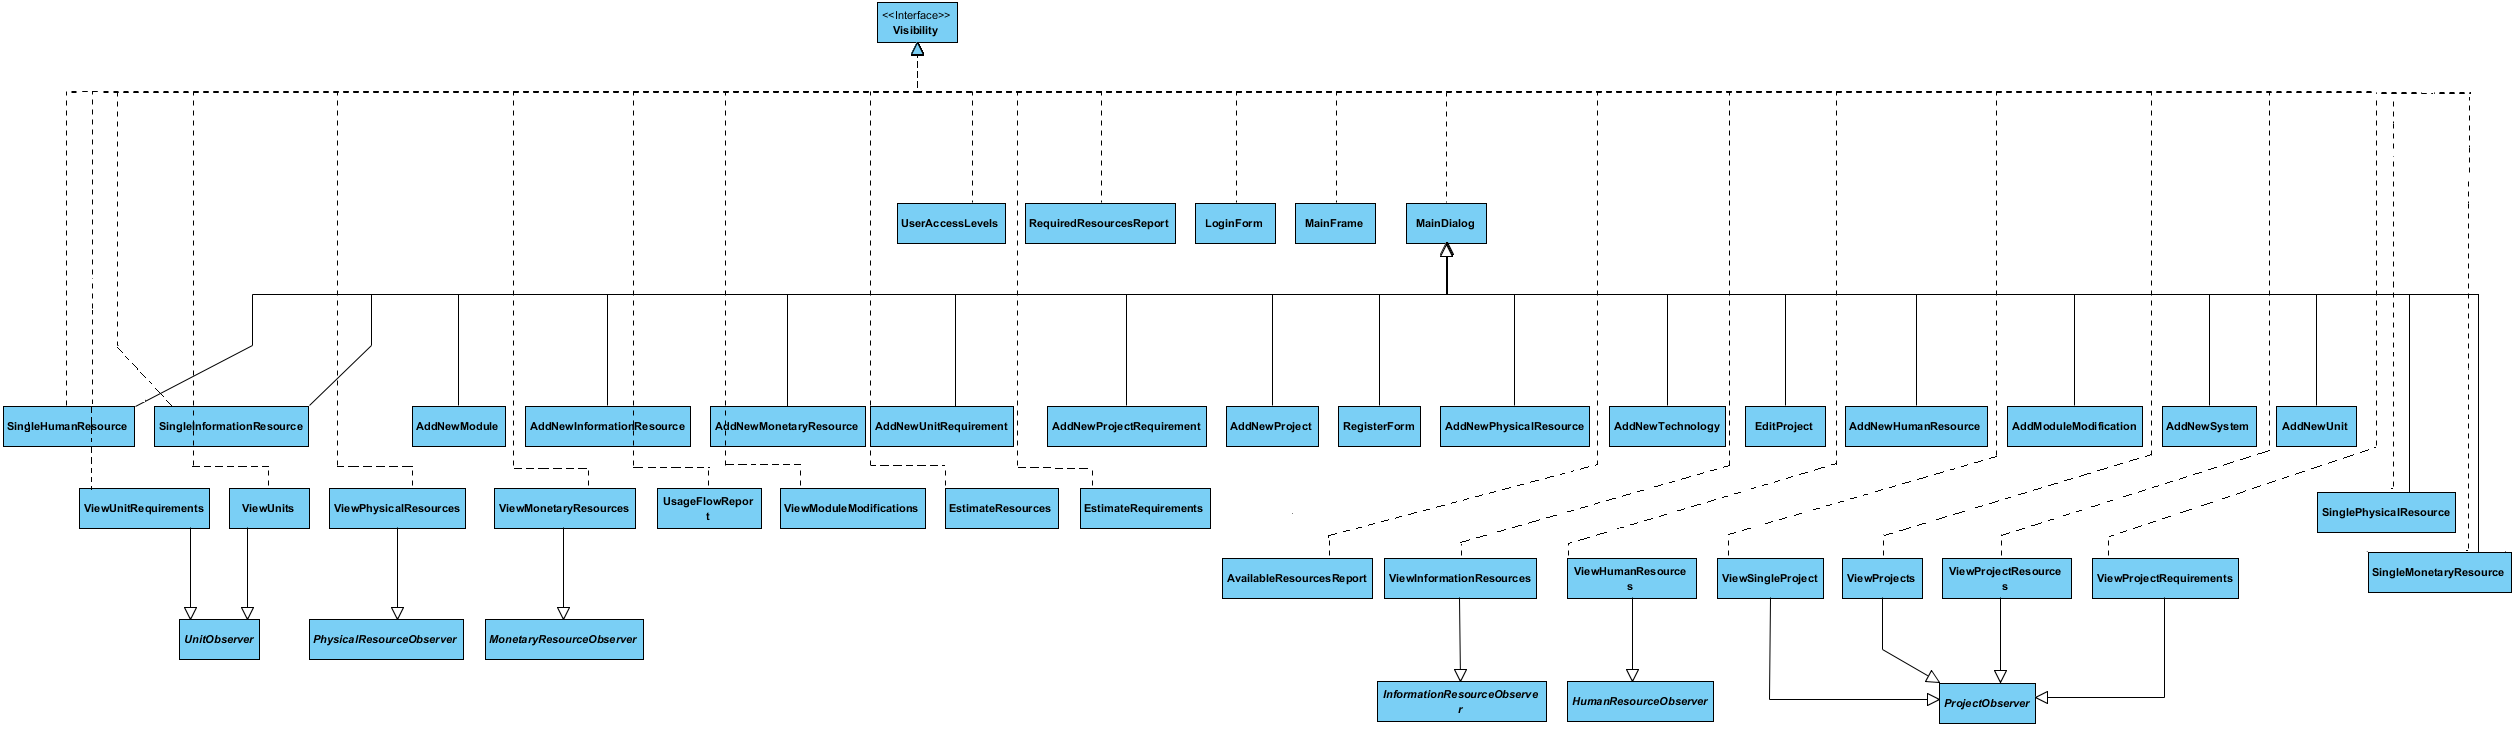
\includegraphics[scale=0.25]{img/class-design/ui/FinalUI}
		\caption{بسته واسط کاربری}
	\end{figure}
\end{landscape}

\subsection{جزییات کلاس‌های واسط کاربری}
\begin{figure}[H]
	\centering
	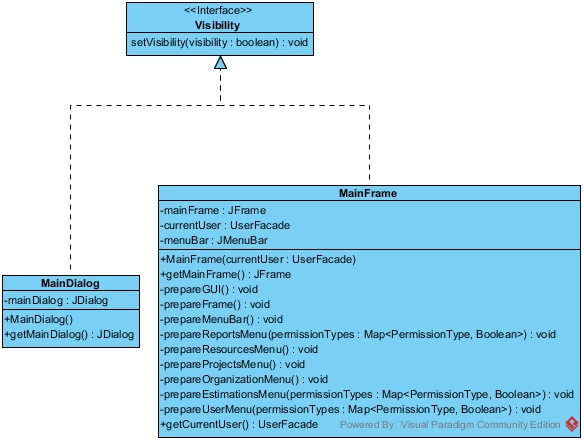
\includegraphics[width=\textwidth]{img/class-design/ui/TopClasses}
	
	\caption{واسط جهت مرئی‌سازی و کلاس‌های سطح بالای اصلی به عنوان قالب اصلی صفحات}
\end{figure}

\begin{figure}[H]
	\centering
	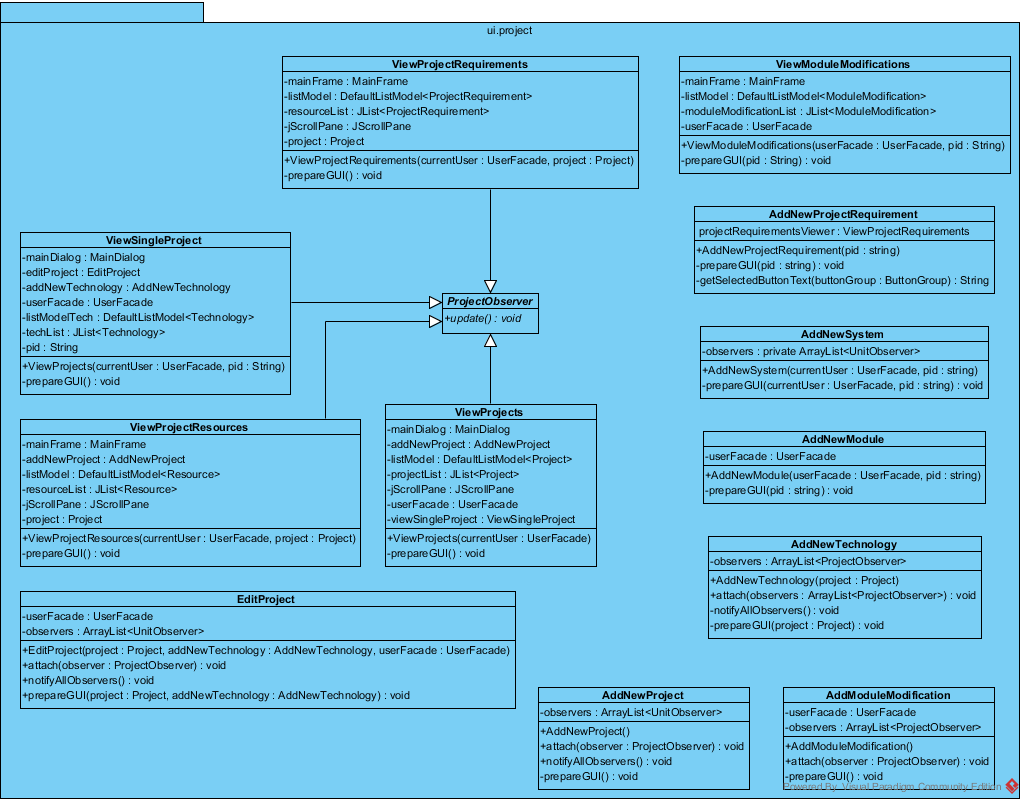
\includegraphics[width=\textwidth]{img/class-design/ui/UIProject}
	
	\caption{بسته‌ی کلاس‌های واسط کاربری پروژه}
\end{figure}

\begin{figure}[H]
	\centering
	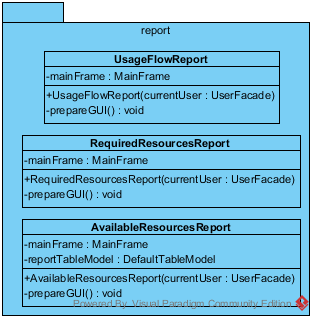
\includegraphics[width=\textwidth]{img/class-design/ui/UIReport}
	
	\caption{بسته‌ی کلاس‌های واسط کاربری گزارش}
\end{figure}

\begin{figure}[H]
	\centering
	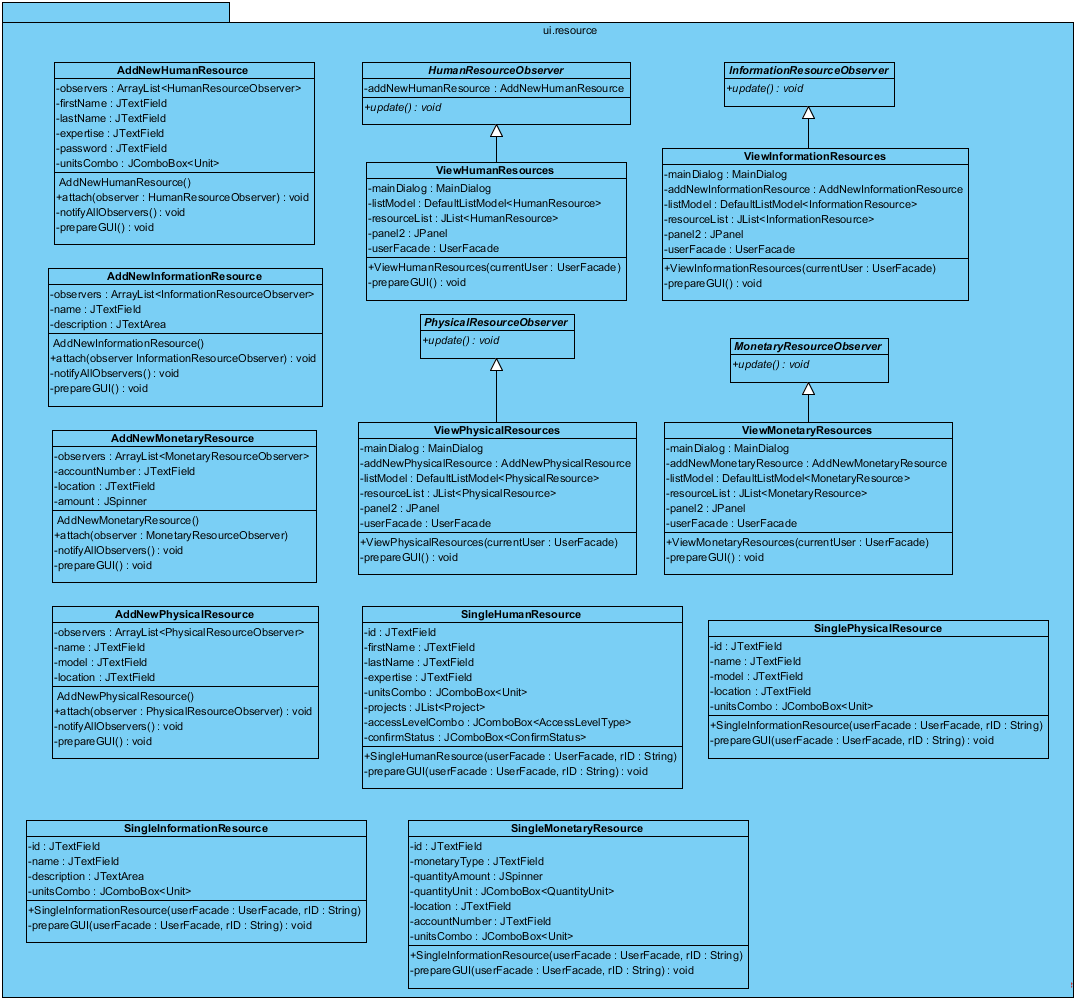
\includegraphics[width=\textwidth]{img/class-design/ui/UIResource}
	
	\caption{بسته‌ی کلاس‌های واسط کاربری منبع}
\end{figure}

\begin{figure}[H]
	\centering
	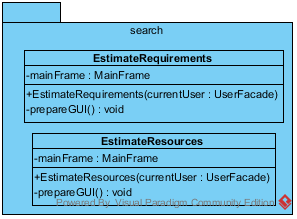
\includegraphics[width=\textwidth]{img/class-design/ui/UISearch}
	
	\caption{جست و جو}
\end{figure}

\begin{figure}[H]
	\centering
	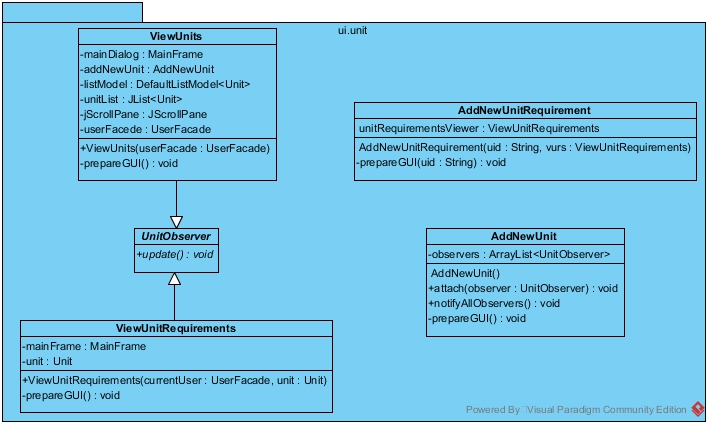
\includegraphics[width=\textwidth]{img/class-design/ui/UIUnit}
	
	\caption{بسته‌ی کلاس‌های واسط کاربری واحد}
\end{figure}

\begin{figure}[H]
	\centering
	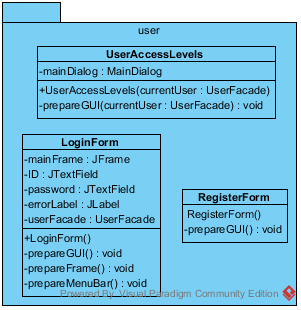
\includegraphics[width=\textwidth]{img/class-design/ui/UIUser}
	
	\caption{بسته‌ی کلاس‌های واسط کاربری کاربر}
\end{figure}
